\chapter{Introduction}
% Introduction section
%  1. Introduction.
%  2. Background and setting. 
%  3. Identification of problem
%  4. Purpose Statement. 
%  5. Objectives or research questions
%  6. Assumptions. Limitations. Definition of terms
%  7. Significance of the study.

% Introduction section (from unsw.edu.au)
% Move A: establish your territory (say what the topic is about)
%   1.  state the general topic and give some background
%   2.  provide a review of the literature related to the topic
%   3.  define the terms and scope of the topic
Optimization plays an important part in our everyday life, science development, product design, and
much more. Examples of optimization could be choosing the optimal way to commute from A to B,
deciding what songs should land on your playlist, or constructing the strongest possible bridge
using limited material. In general, optimization is the methodology of choosing the best decision
among a set of possible decisions. Often we try to quantify how good a decision is: A specific bus
takes 20 min to go from A to B, you rate a specific song 4 out of 5, and a particular bridge design
costs 10 million DKK. Suppose it is possible to come up with a quantification of how good a
decision is in terms of a real number. In that case, we can formluate the optimization problem as
a \textit{mathematical optimization problem}: 
$$\min_{x\in \mathcal{X}} f(x)$$ where the functional $f: \mathcal{X} \rightarrow \mathbb{R}$ is
called the objective function and $\mathcal{X}$ is the set of possible decisions (or decisions you
consider). Note that the optimization problem is formulated as a minimization problem. If one
identifies the optimal decision as a maximum of $f$ (instead of the minima), finding the minima in
the negated objective function $-f(x)$ is equivalent. Throughout this thesis, we refer to
optimization as minimizing the objective function. Solving the mathematical optimization problem is
an active research field, and many algorithms have been developed to find the minimum of the function
$f(\cdot)$.

Evaluation of the objective function can be cheap (e.g., if it just requires summing/multiplying
numbers) or highly expensive (e.g., if it involves human rating, large simulation, or physical
experiments). In the latter case, we want to avoid evaluating the objective function as much as
possible - we want to use \textit{sample-efficient} optimization. The overall topic of this
thesis, \textit{Bayesian optimization}, is one of the preferred frameworks for sample-efficient optimization. 
%maybe mention more?

Bayesian optimization is a probabilistic surrogate-based optimization methodology: Assuming some
initial samples $\{(x_1,f(x_1)), \dots, (x_n,f(x_n))\}$ from a highly expensive objective, a cheap
(surrogate) function is fitted to the samples (in a Bayesian manner). The next sample is found by
minimizing the surrogate, and the process is repeated. Bayesian optimization seeks to enhance this
procedure with probability theory, where the surrogate function becomes a probabilistic (Bayesian)
regression model. The most common surrogate model is a Gaussian Process, as it encapsulates the
uncertainty very well, and its inference procedure (computing answers to probability queries like
$p(y|x)$) is exact.

% Move B: establish a niche (show why there needs to be further research on your topic)
%   4.  outline the current situation
%   5.  evaluate the current situation (advantages/ disadvantages) and identify the gap

Even though GP has proven suitable for many cases, there will be problems where its assumptions do
not hold. For example, the commonly seen GP with an isotropic kernel (covariance between two points
is invariant to translation in input) yields a strong assumption about the continuity of the
objective function and that the objective function behaves similarly throughout the domain
$\mathcal{X}$. However, in Figure \ref{GP_vs_BNN} we see an example of how the GP's uncertainty
quantification is going wild due to a discontinuity in the underlying objective function. in some
areas, it is prevalent to have these discontinuities, for instance, in material discovery, where it
is well known that materials often change very suddenly \cite{Nature_BO_paper}. To accommodate the
strong assumptions of the GP the literature introduces more flexible kernel functions; however, this
introduces additional hyperparameters. Since we often only deal with a small amount of data, tuning
and computation of these more complex GPs can be significantly challenging \cite{Nature_BO_paper}.

\begin{figure}[H]%
    \centering
    \subfloat[\centering GP]{{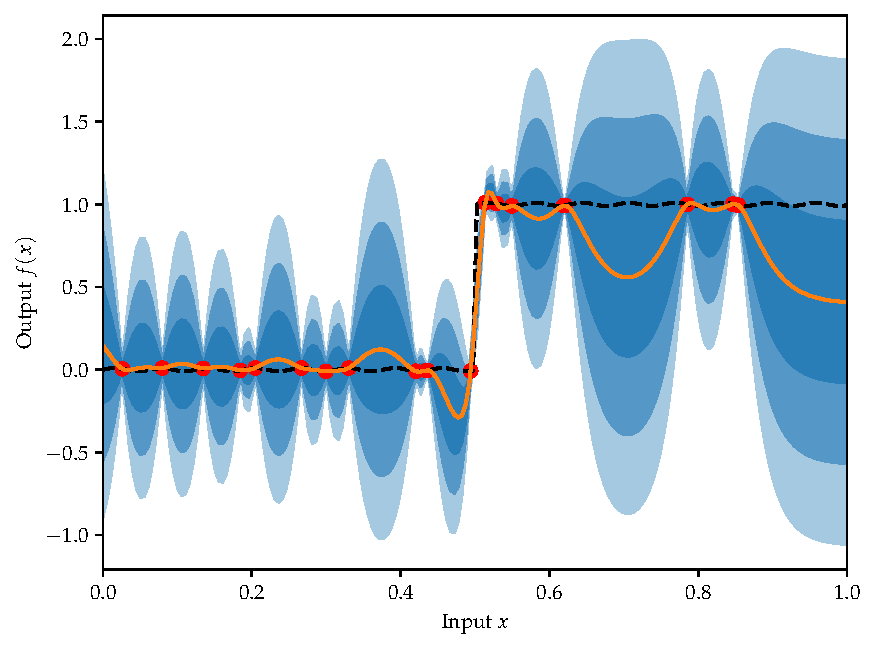
\includegraphics[trim=0.1cm 0.3cm 0.2cm 0.2cm,clip,width=0.46\textwidth]{Pictures/GP_vs_BNN1.pdf} }}%
    \qquad
    \subfloat[\centering BNN]{{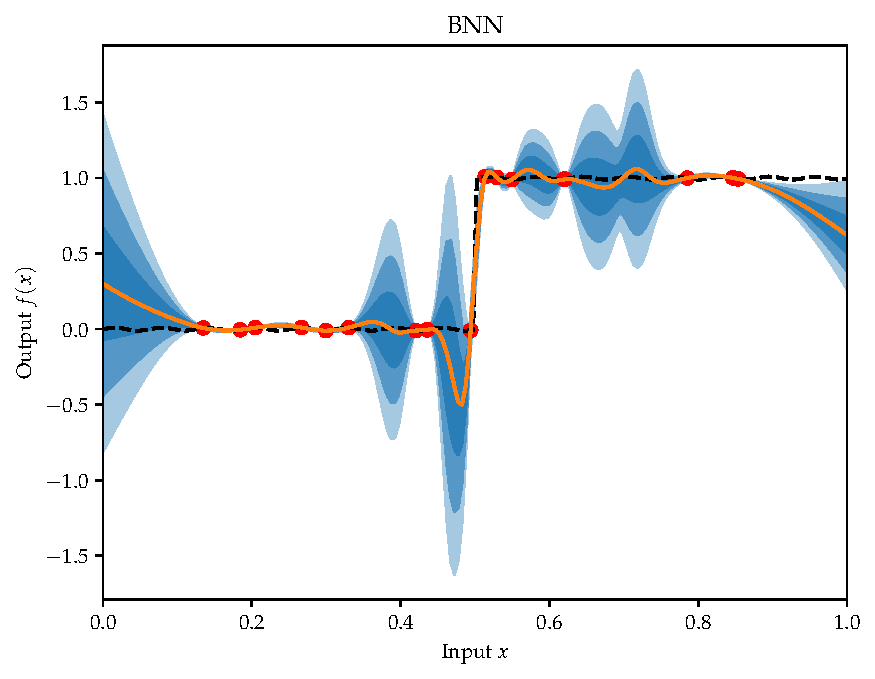
\includegraphics[trim=0.1cm 0.3cm 0.2cm 0.2cm,clip,width=0.46\textwidth]{Pictures/GP_vs_BNN2.pdf} }}%
    \caption{Left: GP fitted to 20 data points. Right: A Bayesian neural network fitted to the same points.
    The objective function is the dashed black line. This examplifies how a discontinuerity makes the 
    standard implemented GP (optimized with emperical bayes) overreact to all other areas in the domain $[0,1]$,
    while the Bayesian NN only express uncertainty where the discontinuerity happen $x = 0.5$}\label{GP_vs_BNN}
\end{figure}


% Move C: introduce the current research (make hypotheses; state the research questions)
%   6.  identify the importance of the proposed research
%   7.  state the research problem/ questions
%   8.  state the research aims and/or research objectives
%   9.  state the hypotheses
%   10. outline the order of information in the thesis
%   11. outline the methodology

GPs are attractive models since they allow for exact inference, a closed-form expected improvement
 (more on this later) and, in general, give a good uncertainty quantification. However, as we saw in
 the figure \ref{fig:GP_vs_BNN} we can maybe do better - especially if we have some insights into
 the behavior of the objective function (i.e. a more transparent the black-box optimization
 problem). Suppose it is possible to evaluate the expensive objective function a few times. Then it
 can potentially save work hours, lots of money, or energy (depending on what makes the objective
 function expensive). It is, therefore, relevant to investigate if other models will perform better.
 As mentioned, the assumptions of GP can be too strong. In this thesis, we aim to create models with
 less strong assumptions, which can perform better on certain classes of (complex) problems, and
 just as well as the GP on most classes of problems. 

%Even though, it would be interesting to also look at different types of GPs such as deep kernel learning
We limit the scope of the project to deal with the following surrogate models, 
\begin{itemize}[noitemsep]
    \item GP with Matérn kernel (Scikit-learn implementation)
    \item Bayesian Neural network (Numpyro implementation)
    \item Bayesian Neural network (BOHAMIANN)
    \item Mixture regression (Gaussian mixture, kernel density estimator, sum-product networks)
\end{itemize}
and we choose only to test the Bayesian optimization with the widely used acquisition function:
\textit{expected improvement}. Furthermore, we only deal with problems in continuous domains
$\mathcal{X} \in \mathbb{R}^m$.

\section{Contribution}
This thesis investigates surrogate models alternative to the isotropic GP - more concretely Bayesian NN
and mixture regression. The proposed hypotheses are,
\begin{enumerate}[noitemsep]
    \item Neural Networks perform better applied to complex BO problems than GPs.
    \item Mixture regression models like SPN can be an effective surrogate model
    performing better than GPs and Neural Networks in some complex cases. 
\end{enumerate}

Note what is meant by performance is \textit{sample efficiency}, i.e., how few evaluations/samples
of the objective function are necessary to find the minima. So here it is assumed that the objective
function is so expensive (whatever that means to the stakeholder) that its cost outweigh the power
and time spend on the surrogate modeling and optimization.


% 1) Firstly, we want to examine what types of problems a GP surrogate is not a good choice and
% where Bayesian neural nets (BNN) surrogates can have an advantage (inspiration found in this 2020
% thesis \cite{PhDthesis})
    
% 2) Looking at sum product networks (SPN) as novel surrogate models. A SPN is - similarly to a BNN
% - a deep probabilistic model and still expressive but with tractable inference, which potentially
% could lead to advantages over BNNs. 

\section{Related work}
Here we give a short overview of research in different surrogates for Bayesian optimization
and the very related field of active learning. The different surrogate models, which are in the 
research we found, 
\begin{itemize}[noitemsep]
    \item Gaussian process
    \item Bayesian neural network
    \item Random forest regression
    \item Kernel density estimator
    \item Bayesian multivariate adaptive regression splines (BMARS)
    \item Bayesian additive regression trees (BART)
\end{itemize}

Since inference time of the GP scales cubic with the number of samples, often research in
alternative surrogate models have its primary focus on lowering the computational complexity of
inference while showing the sample efficiency is (or almost is) as good as the GPs. A popular model
in the current time is a (deep) neural network and using a neural network as a probabilistic
surrogate model (i.e. Bayesian Neural Network \cite{BOHAMIANN} or as basisfunctions in linear
regression \cite{DNGO}) yields only linear complexity. However, as mentioned above, this thesis
assumes that the objective function is always more costly than the inference cost. And cubic
complexity for a GP does not matter for the small number of samples, which is often the case for
highly expensive Bayesian optimization problems. 

Inference complexity is also the main focus of the Ph.D. thesis "Sample-efficient Optimization Using
Neural Networks" from 2020 \cite{PhDthesis}, but his chapter 3 showcases empirically that using Bayesian
neural networks as surrogate models performed better, or at least comparable to GPs on a wide number
of problems. The performance difference was more evident for high-dimensional problems.

The 2021 nature paper "Bayesian optimization with adaptive surrogate models for automated experimental design"
\cite{Nature_BO_paper}, focus on the sample efficiency of the BO applied to autonomous materials discovery, 
which yields a relatively high-dimensional design space and non-smooth patterns of objective functions.  
The paper shows that using Bayesian multivariate adaptive regression splines
and Bayesian additive regression trees as alternative surrogate models outperform GP significantly, 
for complex BO problems. 

Active learning is closely related to Bayesian Optimization, but here the focus is on learning the
underlying function using as few samples as possible instead of just finding its minima. In active
learning, a Gaussian process is also very common, but the paper "Active Learning with Statistical
Models" \cite{ALStatisticalModels} investigates using Gaussian mixtures and kernel estimator in
active learning, i.e. as a surrogate model for selecting the next samples. These are regression
models not seen much in the literature, which is modeling the joint distribution of x and y, and
using the conditional distribution $p(y|x)$ as the regression model. The results were ... ??

\section{Structure of the thesis}
The structure of the thesis is first to build up the foundation around Bayesian optimization, then
present different surrogate/Bayesian regression models, and then results on different types of
problems are shown first on Bayesian regression and next on Bayesian optimization. Finally, a discussion and conclusion. 

\begin{enumerate}[noitemsep]
    \item \textbf{Introduction to Bayesian optimization}, first by establishing its relevance as a
    sample-efficient solver, next by understanding its components: An acquisition function and a 
    surrogate/Bayesian regression model.
    \item \textbf{Discriminative models as surrogates}: Gaussian processes and Bayesian neural
    networks are presented and discussed in terms of inference procedures and regression performance. 
    \item \textbf{Generative(/mixture) models as surrogates}: Since the mixture models are not 
    inherently Bayesian, we present the conditional distribution of in a Bayesian setting. 
    Next, the three different mixture regression models are presented: Kernel density regression, Gaussian mixture regression,
    and the novel (in a regression setting) Sum-product networks.
    \item \textbf{Results} on regression performance and on Bayesian Optimization performance (sample-efficiency)
    \item \textbf{Discussion} and \textbf{conclusion}
\end{enumerate}

% \begin{itemize}
%     \item The first chapter introduces the concept of optimization in general, Bayesian optimization 
%     and how surrogates/Bayesian regression models are relevant.
%     \item The second chapter introduces GP and Bayesian Neural Networks
%     \item The third chapter introduces the mixture regression and the novel SPN regression.
%     \item The fourth chapter results
%     \item Finally a discussion and conclusion.
% \end{itemize}


\section{notation}
Throughout this thesis we will be using Bayesian notation, i.e. $p(x) := P(X=x)$ is the probability
density function of the random variable $X$ evaluated in $x$. and $p(y|x) := P(Y=y|X=x)$ or $p(y|x)
:= P(Y|X=x)$. And writing $p(y^2|x)$ means $P(Y^2=y^2|X=x)$ and \textbf{not} $P(Y=y^2|X=x)$

The density of a normal distribution evaluated in $x$ is denoted as, $\mathcal{N}(x|\mu, \Sigma)$. 

We will not distinguish between vectors and scalars notation-wise unless it is not clear from the 
context. 

% We refer to the "Optimization landscape" defined as the joint set of points in the domain and the objective function
% evaluated in the points, i.e. $\{(x,f(x))\in \mathcal{X} \times \mathbb{R}| x \in \mathcal{X}\}$
